\chapter{Hardware Design and Implementation}
    \section{Micro-architecture Design}
        In this section, we will look into DeAr from a micro-architecture perspective, and explore its design considerations at the same time.
        DSP designers usually evaluate the computing power of a DSP by Million Operations per Second (MOPS).
        Conventionally, the clock speed and SIMD width (number of lanes) of DSP are the main determinant of MOPS.
        Unfortunately, owing to the limits of CMOS technology and the significant growth of bus complexity, 
        driving the clock speed or increasing the SIMD width are consequently infeasible.
        Instead, the we adopted the concept of VLIW, which is able to issue multiple operations in a cycle.
        One of the key features of the proposed DeAr datapath is manipulating Simultaneous Multi-threading (SMT) in each DSP lane to exploit the arithmetic resources.
        By scheduling DeAr threads for the collaborative execution, the workload of each work-item can be shared by two concurrent DeAr threads, 
        which accelerate the execution of the wavefront and gain higher MOPS without touching the clock speed or SIMD width.
        Another one is exhaustively compacting the hardware resources while keeping the flexibility and computation power.
        This offers the DeAr dataptah better efficiency in several perspectives, such as power consumption, chip area and code storage.
        \\\indent
        Figure~\ref{fig:micro} illustrates the micro-architecture of DeAr datapath applied in each DSP lane.
        Two DeAr threads residing in a lane share a group of arithmetic units that commonly exist in a RISC datapath.
        The demonstrated example includes an adder, a multiplier and a barrel shifter, which are qualified to perform most benchmarks,
        Nevertheless, the configuration of arithmetic units can be modified to fit the target applications.
        The output of each arithmetic unit is an accumulator register, 
        which bypasses the result to any arithmetic units that need it in the next clock cycle.
        The bypassing-mechanism of accumulator registers avoid unnecessary accesses to RF, 
        and thus reduce the energy dissipation in RF.
        In addition, the accumulator registers are all clock-gated.
        This enables DeAr to preserve the data in accumulator registers until the corresponding arithmetic unit is activated next time, 
        offering more data bypassing opportunities.
        The bypassing mechanism and resolution of structural hazards are both handled by the software, 
        so the hardware complexity of dynamic scheduling or bypassing units can be avoided or reduced.
        \\\indent
        The RF is physically and symmetrically separated for two DeAr threads.
        Each of them owns a pair of private queue memories as well as a private stack memory, 
        and these memory units of two DeAr threads form the sequential-accessed banked RF.
        The banked organization of the RF cuts off redundant connectivity among read/write ports and register cells.
        Compared with the conventional centralized organization, 
        the wire area, power consumption and access time of the banked organization are significantly improved, 
        The queue pair, composed of an load-queue and store-queue, 
        serves as the buffer that interfaces the lower level of the memory hierarchy with the datapath.
        Load-queues and store-queues are accessed from their both sides concurrently in the first-in-first-out (FIFO) fashion.
        The DeAr thread reads input data from its load-queue and writes the result of computation to its store-queue, 
        while the load/store unit accesses the queues in the opposite direction.
        By preventing the queues from empty or full with clever scheduling, the latency of load/store can thus be hidden.
        The stack memory, on the other hand, is responsible for the storage of intermediate data.
        The nature of a stack memory is last-in-first-out (LIFO), 
        which is the key property of the DeAr scheduling algorithm (elaborated in Chapter~\ref{cha:software}).
        Using the sequential-access memory rather than a random-access one in RF effectively reduces the length of control signal, 
        since any access to RF can be simplified to "Push" or "Pop".
        The reduction in the length of control signal gains high code density and save the wiring from the instruction unit to RF.
        This is the key advantage of DeAr over conventional VLIW architectures.
        \\\indent
        The compact data bus separates the RF and arithmetic units with a set of multiplexers controlled by the instruction unit.
        Figure~\ref{fig:databus} reveals the details of the compact data bus, 
        We can summarize the route of data as below:
        \begin{itemize}
            \item Each arithmetic unit receives the first operand from a load-queue or an accumulator.
        and receives the second one (if exists) from a load-queue or a stack.
            \item Each store-queue receives data from the output of an arithmetic unit.
            \item Each stack receives data from the output of an arithmetic unit.
        \end{itemize}
        It is important to note that, even though the communication among the RF, arithmetic units and accumulator registers is compacted exhaustively, 
        the flexibility of the datapath is still be kept.
        By such a compact design of the data bus, the further reduction in the length of control signal can be achieved.
        \vspace{\textfig}
        \begin{figure}[!ht] 
            \centering
            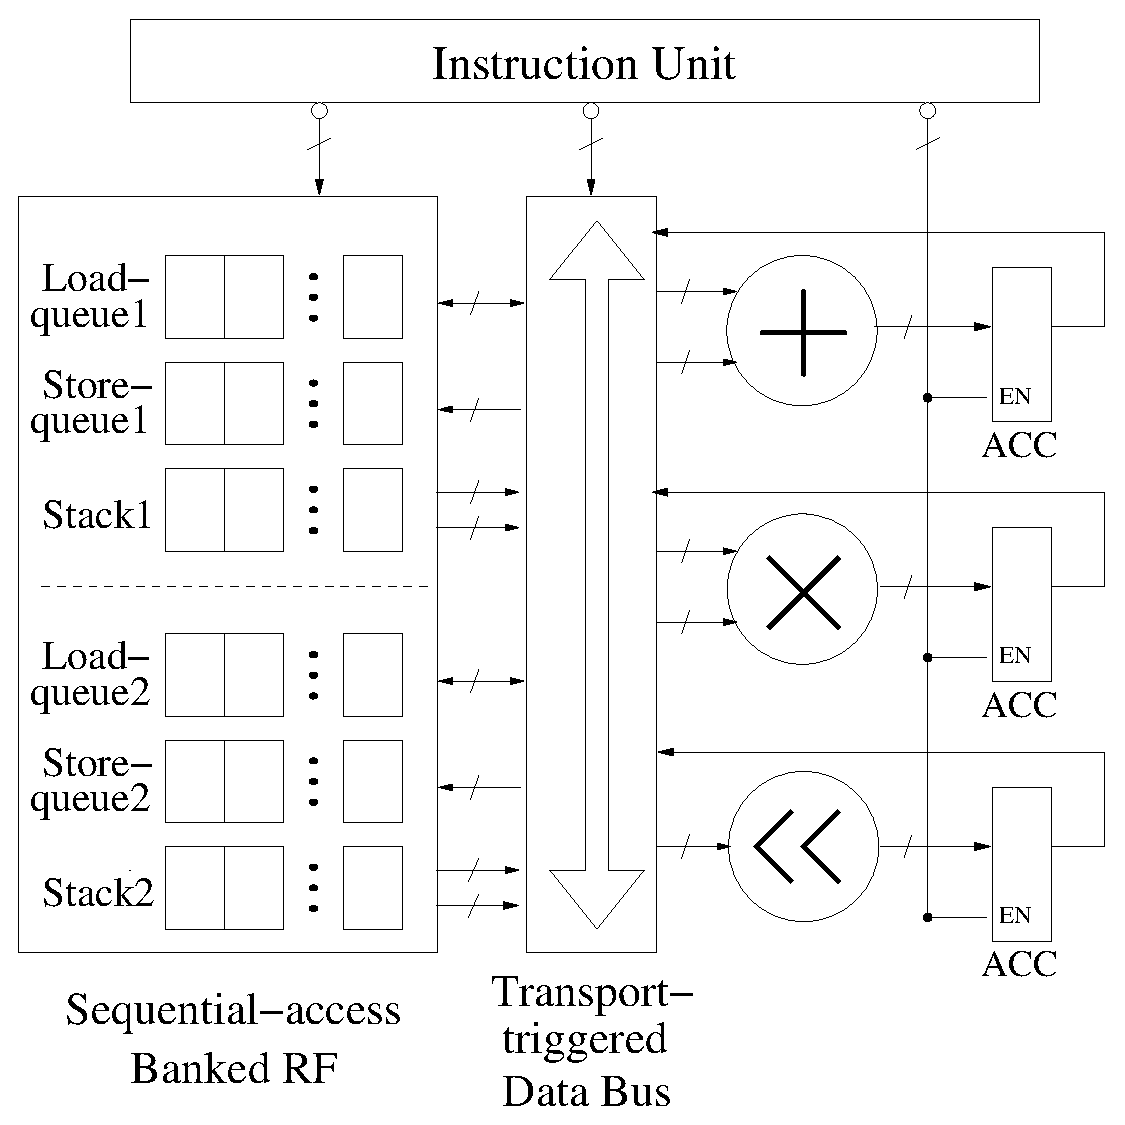
\includegraphics[width=0.85\textwidth]{./figs/micro.eps}
            \caption{Micro-architecture of a DeAr DSP lane}
            \label{fig:micro}
        \end{figure}

    \section{Instruction Set Architecture}

    %---------- risc-style portion table
    \begin{table}[ht!]
        \centering
        \begin{tabular}{|c|l|l|c|}
            \hline
        \multicolumn{1}{|c|}{\textbf{Category}} & \multicolumn{1}{c|}{\textbf{Name}} & \multicolumn{1}{c|}{\textbf{Meaning}} & \multicolumn{1}{c|}{\textbf{\begin{tabular}[c|]{@{}c@{}}Followed \\ by stack \\ operation?\end{tabular}}} \\ \hline
            \multirow{5}{*}{Arithmetic}    & Add & \textbf{d} = \textbf{s} + \textbf{t} & \multirow{7}{*}{Yes}  \\ \cline{2-3}
                                           & Subtract & \textbf{d} = \textbf{s} - \textbf{t} & \\ \cline{2-3} 
                                           & Multiply & \textbf{d} = \textbf{s} * \textbf{t} & \\ \cline{2-3} 
                                           & Shift left & \textbf{d} = \textbf{s} << \textbf{t} & \\ \cline{2-3}
                                           & Shift right & \textbf{d} = \textbf{s} >> \textbf{t} & \\ \cline{1-3}
            \multirow{2}{*}{Others}        & Move & \textbf{d} = \textbf{s} + 0 or \textbf{d} = \textbf{s} << 0 & \\ \cline{2-3} 
                                           & Nop & no operation & \\ \hline
            \multirow{2}{*}{Memory transfer} & Load burst & repeat(\textbf{b}) load\_queue.push (memory[\textbf{a}]) & \multirow{2}{*}{No} \\ \cline{2-3} 
                                             & Store burst & repeat(\textbf{b}) memory[\textbf{a}] = store\_queue.pop() & \\ \hline
        \end{tabular}
        \caption{RISC-style portion of the DeAr instruction set}
        \label{my-label}
    \end{table}
    %-----------------------------------------
    %---------- stack portion table
\begin{table}[ht!]
\centering
\begin{tabular}{|l|l|l|}
    \hline
    \multicolumn{1}{|c|}{\textbf{Name}} & \multicolumn{1}{c|}{\textbf{Meaning}} & \multicolumn{1}{c|}{\textbf{Note}} \\ \hline
    Push & \begin{tabular}[c]{@{}l@{}}1. Add the head address by 1\\ 2. Write the new data to the head address\end{tabular} & \multirow{2}{*}{ \parbox{5cm}{A "pop" followed by a "push" is equivalent to a "modify"} } \\ \cline{1-2}
    Pop                               & \begin{tabular}[c]{@{}l@{}}1. Subtract the head address by 1\\ 2. Invalidate the previous head data\end{tabular} & \\ \hline
    Modify                            & Modify the head data to to the new data & The head address remains \\ \hline
    Nop                               & No operation & The head address and data remain \\ \hline
    \end{tabular}
\caption{Stack access portion of the DeAr instrucion set}
\label{tab:stack}
\end{table}
    %-----------------------------------------


    \section{System Integration}
